\documentclass[journal,12pt,twocolumn]{IEEEtran}

\usepackage{enumitem}
\usepackage{amsmath}
\usepackage{amssymb}
\usepackage{gensymb}
\usepackage{graphicx}
\usepackage{txfonts}         
\usepackage{listings}
\usepackage{lstautogobble}
\usepackage{mathtools}

\newcommand{\solution}{\noindent \textbf{Solution: }}
\providecommand{\pr}[1]{\ensuremath{\Pr\left(#1\right)}}
\providecommand{\brak}[1]{\ensuremath{\left(#1\right)}}
\providecommand{\cbrak}[1]{\ensuremath{\left\{#1\right\}}}
\providecommand{\sbrak}[1]{\ensuremath{\left[#1\right]}}
\providecommand{\mean}[1]{E[ #1 ]}
\providecommand{\var}[1]{\mathrm{Var}[ #1 ]}
\providecommand{\der}[1]{\mathrm{d} #1}
\providecommand{\gauss}[2]{\mathcal{N}\ensuremath{\left(#1,#2\right)}}

\let\StandardTheFigure\thefigure
\let\vec\mathbf

\numberwithin{equation}{section}
\renewcommand{\thefigure}{\theenumi}
\renewcommand\thesection{\arabic{section}}

\newcommand{\myvec}[1]{\ensuremath{\begin{pmatrix}#1\end{pmatrix}}}
\newcommand{\mydet}[1]{\ensuremath{\begin{vmatrix}#1\end{vmatrix}}}

\lstset {
	frame=single, 
	breaklines=true,
	columns=fullflexible,
	autogobble=true
}            
                               
\title{Random Numbers \\
\Large AI1110: Probability and Random Variables}\\
\author{YASH R RAMTEKE \\ \normalsize BT21BTECH11006\\ \vspace*{20pt} \normalsize  8 JULY 2022}

\begin{document}

	\maketitle
	
	\section{Uniform Random Numbers}
	Let $U$ be a uniform random variable between 0 and 1.
	\begin{enumerate}[label=\thesection.\arabic*,ref=\thesection.\theenumi]
	\item Generate $10^6$ samples of $U$ using a C program and save into a file called uni.dat

	\solution Download the C source code by executing the following commands
	\begin{lstlisting}
		wget https://raw.githubusercontent.com/gadepall/AI1110/main/sim/codes/exrand.c
		wget https://raw.githubusercontent.com/gadepall/AI1110/main/sim/codes/coeffs.h
	\end{lstlisting}
	Compile and run the C program by executing the following
	\begin{lstlisting}
		gcc exrand.c
		./a.out
	\end{lstlisting}
	
	\item Load the uni.dat file into Python and plot the empirical CDF of $U$ using the samples in uni.dat. The CDF is defined as
	\begin{align}
		F_{U}(x) = \pr{U \le x}
	\end{align}
	
	\solution  Download the following Python code that plots Fig. \ref{fig-1_2}
	\begin{lstlisting}
wget https://raw.githubusercontent.com/YashRRamteke/Random-numbers/main/Code/cdf_plot.py
python3 cdf_plot.py
	\end{lstlisting}
	\begin{figure}
		\centering
		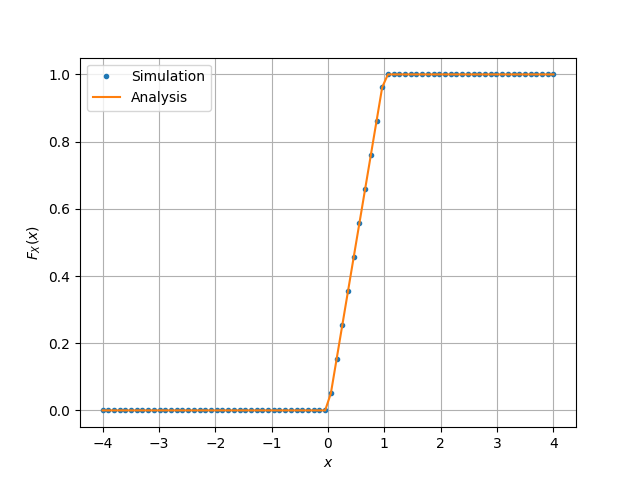
\includegraphics[width=\columnwidth]{1_2.png}
		\caption{The CDF of $U$}
		\label{fig-1_2}
	\end{figure}
	
	\item
Find a  theoretical expression for $F_{U}(x)$.
\\
\solution
$U$ is given by 
\begin{align}
    U(x) = 
    \begin{cases}
        0, & x \in (-\infty,0) \\
        1, & x \in (0,1) \\
        0, & x \in (1, \infty)
    \end{cases}
\end{align}
Therefore, we have:
    \begin{align}
        F_U(x) = \int_0^x U(x) dx
    \end{align}
Computing the integral, we get:
\begin{align}
    F_U(x) = 
    \begin{cases}
        0, & x \in (-\infty,0) \\
        x, & x \in (0,1) \\
        1, & x \in (1, \infty)
    \end{cases}
\end{align}

\item
The mean of $U$ is defined as
%
\begin{equation}
E\sbrak{U} = \frac{1}{N}\sum_{i=1}^{N}U_i
\end{equation}
%
and its variance as
%
\begin{equation}
\text{var}\sbrak{U} = E\sbrak{U- E\sbrak{U}}^2 
\end{equation}

Write a C program to  find the mean and variance of $U$.
\\
\solution
Add the following function to coeffs.h
\begin{lstlisting}
double variance(char *str)
{
int i=0,c;
FILE *fp;
double x, temp=0.0;
fp = fopen(str,"r");
//get numbers from file
while(fscanf(fp,"%lf",&x)!=EOF)
{
//Count numbers in file
i=i+1;
//Add all numbers in file
temp = temp+x*x;
}
double mn = mean(str);
fclose(fp);
temp = temp/(i-1);
return temp - mn*mn ;
}
    \end{lstlisting}
Following the steps mentioned below gives the required result:
\begin{lstlisting}
    gcc exrand.c
    ./a.out
    mean = 0.500031
    variance = 0.083247
\end{lstlisting}


\item Verify your result theoretically given that
\end{enumerate}
%
\begin{equation}
E\sbrak{U^k} = \int_{-\infty}^{\infty}x^kdF_{U}(x)
\end{equation}
\\
\solution  Since 
\begin{align}
    dF_U(x) = p_U(x) dx
\end{align}
we have:
\begin{align}
    \label{eq2}
    E[U^k] = \int_{-\infty}^{\infty}x^k p_U(x) dx
\end{align}
Also,
\begin{align}
    \label{eq3}
     p_U(x) = 
    \begin{cases}
        0, & x \in (-\infty,0) \\
        1, & x \in (0,1) \\
        0, & x \in (1, \infty)
    \end{cases}
\end{align}
Therefore, from Equations \ref{eq2} and \ref{eq3}, we have:
    
    \begin{align}
        E[U^2] &=  \int_{-\infty}^{\infty}x^2 p_U(x) dx \\
        &= \int_0 ^1 x^2 dx \\
        &= \frac{1}{3}
    \end{align}
    
    Similarly, 
    \begin{align}
        E[U] &=  \int_{-\infty}^{\infty}x p_U(x) dx \\
        &= \int_0 ^1 x dx \\
        &= \frac{1}{2}
    \end{align}
    Therefore, the mean is $\frac{1}{2}$, and the variance equals:
    \begin{align}
        E[U^2] - E[U]^2 &= \frac{1}{3} - \brak{\frac{1}{2}}^2 \\
        &= \frac{1}{12}
    \end{align}
    
\section{Central Limit Theorem}
%
\begin{enumerate}[label=\thesection.\arabic*
,ref=\thesection.\theenumi]

\item
Generate $10^6$ samples of the random variable
%
\begin{equation}
X = \sum_{i=1}^{12}U_i -6
\end{equation}
%
using a C program, where $U_i, i = 1,2,\dots, 12$ are  a set of independent uniform random variables between 0 and 1
and save in a file called gau.dat
\\
\solution
Add the following line to \textbf{exrand.c} and execute the code:
\begin{lstlisting}
    gaussian("gau.dat", 1000000);
    gcc exrand.c
    ./a.out
\end{lstlisting}

\item
Load gau.dat in python and plot the empirical CDF of $X$ using the samples in gau.dat. What properties does a CDF have?
\\
\begin{lstlisting}
wget https://raw.githubusercontent.com/YashRRamteke/Random-numbers/main/Code/cdf_plot.py
\end{lstlisting}
and execute it with
\begin{lstlisting}
python3 cdf_plot.py
\end{lstlisting}

\begin{figure}
\centering
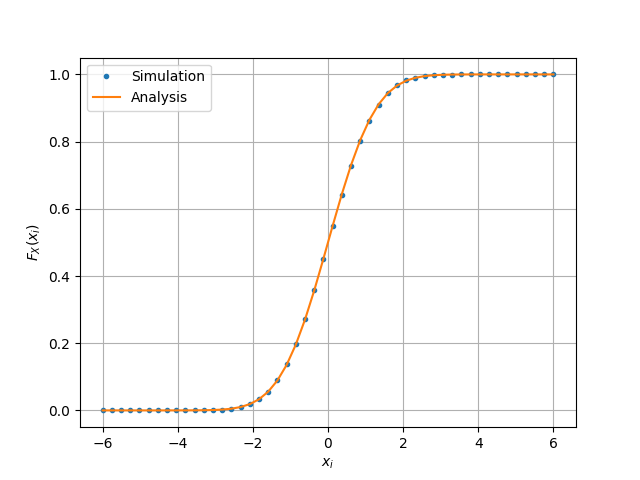
\includegraphics[width=\columnwidth]{2_2.png}
\caption{The CDF of $X$}
\label{fig:gauss_pdf}
\end{figure}

The CDF of a probability distribution has the following properties:
		\begin{enumerate}
			\item It is non-decreasing
			\item It is right-continuous
			\item $\lim_{x \to -\infty}F_X(x) = 0$
			\item $\lim_{x \to \infty}F_X(x) = 1$
		\end{enumerate}
The CDF of the normal distribution is expressed in terms of the Q-function as\\ $F_X(x) = 1 - Q(x)$.


\item
Load gau.dat in python and plot the empirical PDF of $X$ using the samples in gau.dat. The PDF of $X$ is defined as
\begin{align}
p_{X}(x) = \frac{d}{dx}F_{X}(x)
\end{align}
What properties does the PDF have?
\\
\solution The PDF of $X$ is plotted in Fig. \ref{fig:gauss_pdf} using the code below
\begin{lstlisting}
wget https://raw.githubusercontent.com/YashRRamteke/Random-numbers/main/Code/pdf_plot.py
python3 pdf_plot.py
\end{lstlisting}
\begin{figure}
\centering
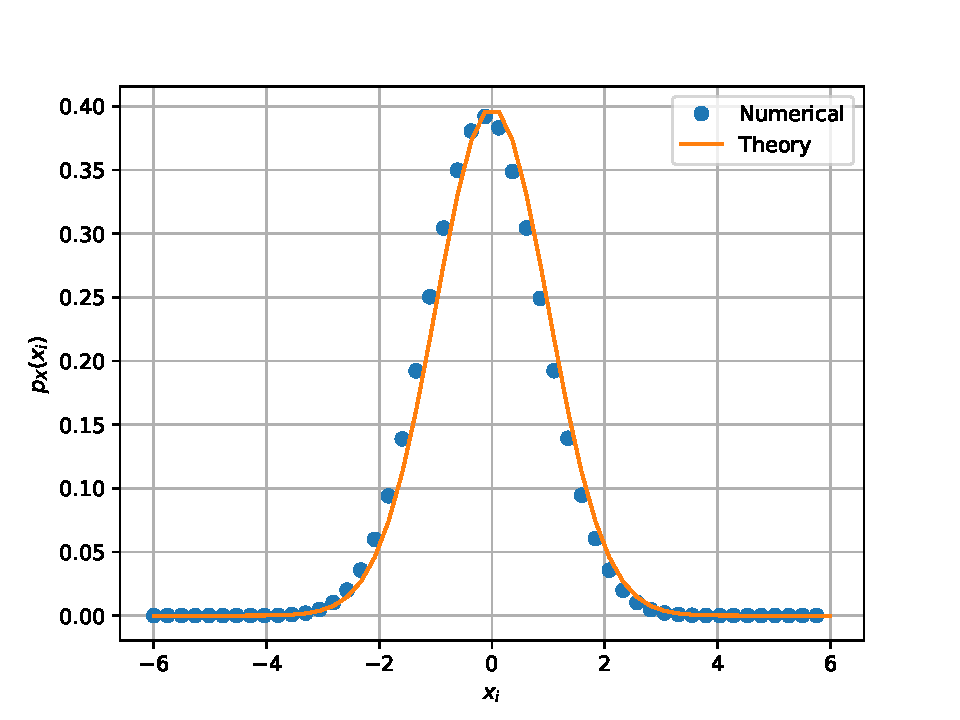
\includegraphics[width=\columnwidth]{gauss_pdf.pdf}
\caption{The PDF of $X$}
\label{fig:gauss_pdf}
\end{figure}

\item Find the mean and variance of $X$ by writing a C program.
\\
\solution Use the main and variance functions in \textbf{coeffs.h}, and execute the code below
\begin{lstlisting}
    gcc exrand.c
    ./a.out
\end{lstlisting}
We get
\begin{lstlisting}
    mean = 0.000685
    variance = 1.000025
\end{lstlisting}


\item Given that 
\begin{align}
p_{X}(x) = \frac{1}{\sqrt{2\pi}}\exp\brak{-\frac{x^2}{2}}, -\infty < x < \infty,
\end{align}
repeat the above exercise theoretically.
\\
\solution  We have:
    
\begin{align}
    E[X] &=  \int_{-\infty}^{\infty} \frac{x}{\sqrt{2\pi}}\exp{\left(-\frac{x^2}{2}\right)} \\
    &= -\frac{1}{\sqrt{2\pi}}\exp\brak{-\frac{x^2}{2}} \Bigg{|}_{-\infty}^{\infty} \\
    &= 0 
\end{align}
Also,
    
\begin{align}
    E[X^2] &=  \int_{-\infty}^{\infty} \frac{x^2}{\sqrt{2\pi}}\exp{\left(-\frac{x^2}{2}\right)} \\
    &= -\frac{x}{\sqrt{2\pi}}e^{\brak{-\frac{x^2}{2}}} \Bigg{|}_{-\infty}^{\infty} + \int_{-\infty}^{\infty} \frac{1}{\sqrt{2\pi}}e^{\brak{-\frac{x^2}{2}}}   \\
    &= 0 + \frac{1}{\sqrt{2\pi}} \times \sqrt{2\pi} \\
    &= 1
\end{align}
Hence, 
\begin{align}
    \text{var}(X) &= E[X^2] - E[X]^2 \\ 
    &= 1 
\end{align}
Therefore, the mean is $0$ and the variance is $1$. Running the empirical code in \textbf{./Code/exrand.c}, 
   we get mean = $0.000685$ and variance = $1.000025$, which closely matches the theoretical values.
   

\item Find the theoretical CDF of $X$
\\
\solution
 To find the theoretical CDF, consider:
\begin{align}
    Q_X(x) &= \int_x ^{\infty} \frac{1}{\sqrt{2\pi}} e^{\frac{-x^2}{2}} dx \\
      &= \frac{\text{erfc}(\frac{x}{\sqrt{2}})}{2}
   \end{align}
The CDF is then:
\begin{align}
    F_X(x) &= 1 - Q_X(x) \\
    &= 1 - \frac{\text{erfc}(\frac{x}{\sqrt{2}})}{2}
\end{align}

\section{From Uniform to Other}
\begin{enumerate}[label=\thesection.\arabic*
,ref=\thesection.\theenumi]
%
\item
Generate samples of 
%
\begin{equation}
V = -2\ln\brak{1-U}
\end{equation}
%
and plot its CDF.  
\solution 
Add the following function to \textbf{coeffs.h}:
\begin{lstlisting}
    void logarithmic(char *str){
  int i=0,c;
FILE *fp, *fp2;
double x, temp=0.0;
fp = fopen("uni.dat","r");
fp2 = fopen(str, "w");
//get numbers from file
while(fscanf(fp,"%lf",&x)!=EOF)
{
  temp = -2*log(1-x);
  fprintf(fp2,"%lf\n",temp);
}
fclose(fp);
fclose(fp2);
return ;
}
    \end{lstlisting}
Using this function in \textbf{exrand.c} prints the numbers in 
\textbf{log.dat} 


\item Find a theoretical expression for $F_V(x)$.
\\
\solution  We have:
    
\begin{align}
F_V(x) &= \pr{V \leq x} \\
&= \pr{-2\ln(1-U) \leq x} \\
&= \pr{1-U \geq	\exp{\left(-\frac{x}{2}\right)}} \\
&= \pr{U \leq 1 - \exp{\left(-\frac{x}{2}\right)}} \\
&= F_U\left(1 - \exp{\left(-\frac{x}{2}\right)}\right) 
\end{align}
Therefore,
    \begin{align}
       F_V(x) =
        \begin{cases}
            0, & 1 - \exp{\left(-\frac{x}{2}\right)} \in (-\infty,0) \\
            1 - \exp{\left(-\frac{x}{2}\right)}, & 1 - \exp{\left(-\frac{x}{2}\right)} \in (0,1) \\
            1, & 1 - \exp{\left(-\frac{x}{2}\right)} \in (1, \infty)
        \end{cases}
    \end{align}
    
    From this we get:
    
    \begin{align}
       F_V(x) =
        \begin{cases}
            0, & x \in (-\infty,0) \\
            1 - \exp{\left(-\frac{x}{2}\right)}, & x \in (0,\infty) 
        \end{cases}
    \end{align}
    \begin{figure}
        \centering
        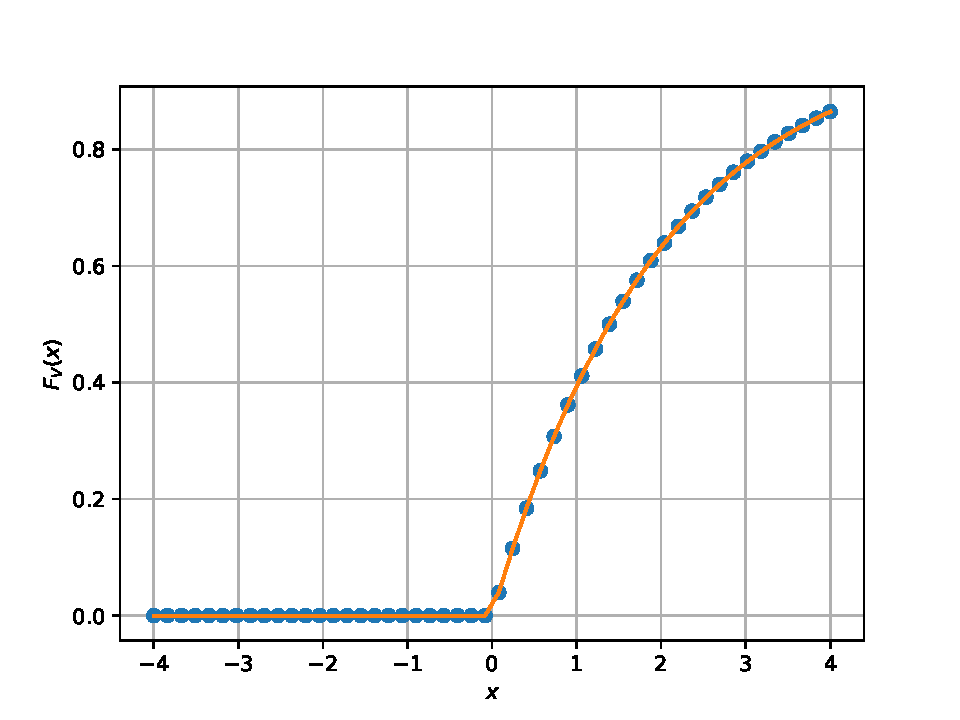
\includegraphics[width=\columnwidth]{V_cdf.pdf}
        \caption{The CDF of $V$}
        \label{fig:V_cdf.pdf}
        \end{figure}
    The CDF of $V$ is plotted in Fig. 3.2
%
%\item
%Generate the Rayleigh distribution from Uniform. Verify your result through graphical plots.
    \end{enumerate}


\end{enumerate}

\end{document}
